%----------------------------------------------------------
Esta parte del algoritmo tiene como objetivo extraer información de las imágenes que captura el UAV. Para ello nos basamos en el algoritmo de segmentación por color de CMU \cite{JamesBruce_CMU_SEG}.  \\

\begin{figure}[h]
	\centering
	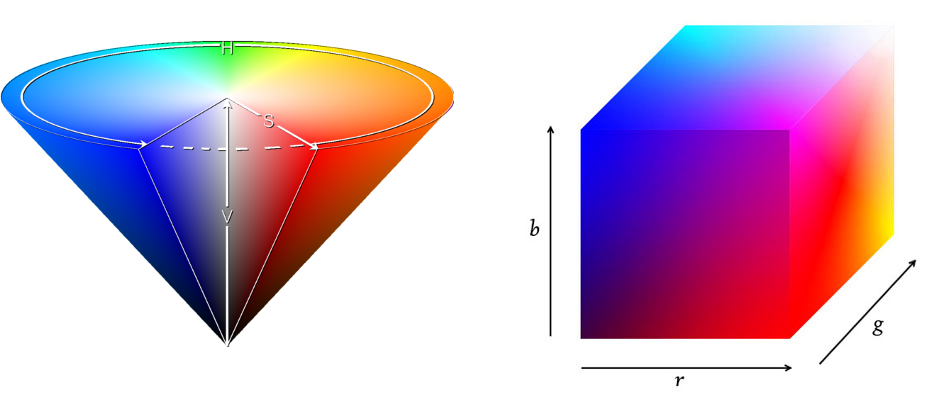
\includegraphics[width=0.75\textwidth,natwidth=944,natheight=400]{../Images/c2/HSV_vs_RGB.png}
	\caption{Espacios de colores HSV y RGB}
	\label{fig:HSV_vs_RGB}
\end{figure}

Se divide el espacio de colores tal que se puedan seleccionar en función de este las diferentes partes de la imagen y luego se agrupan los cl\'usteres de colores para formar un solo objeto. \\

La siguiente figura muestra un ejemplo de la ejecuci\'on del algoritmo.

\begin{figure}
        \centering
        \begin{subfigure}[b]{0.4\textwidth}
	        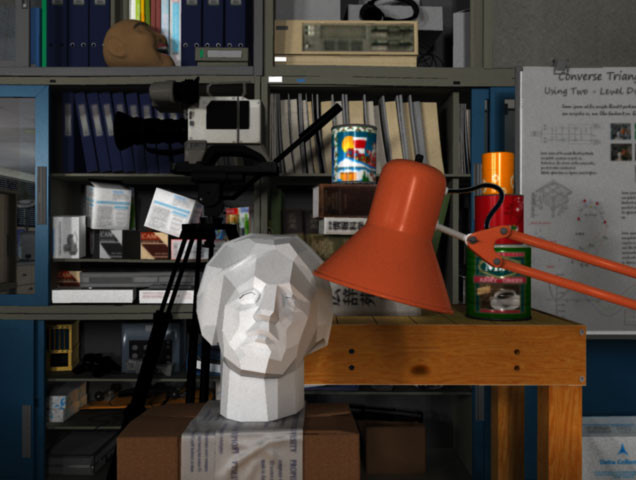
\includegraphics[width=\linewidth]{../Images/c2/head_scene_tsukuba_ori}
        	\caption{Original}
        	\label{fig:head_scene_tsukuba_ori}   
        \end{subfigure}%
        ~
        \begin{subfigure}[b]{0.4\textwidth}
            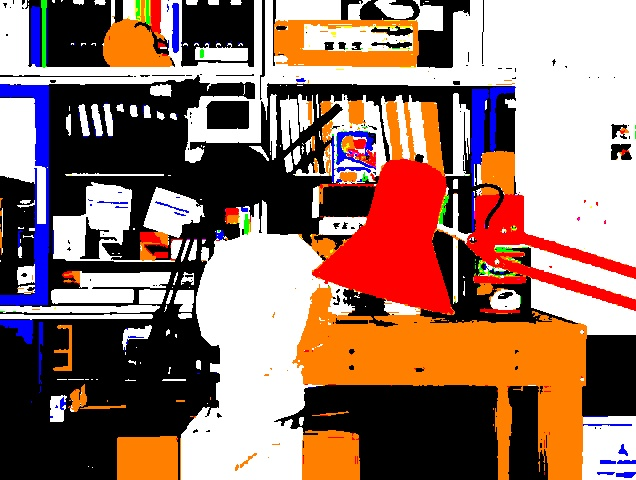
\includegraphics[width=\linewidth]{../Images/c2/head_scene_tsukuba_seg}
           	\caption{Segmentada}
           	\label{fig:head_scene_tsukuba_seg}
        \end{subfigure}
        \caption{$Head Scene$}
\end{figure}

